\receta{Spaguetti con Verduras y Especias}

Esta es una receta de mi hermano, que salió de su propia inspiración y le salió bastante buena, la recomiendo mucho.\\

Rinde para 3 personas.\\

\begin{ingredientes}
\item 250g Spaguetti
\item 400g Pimentón
\item 520g Calabazin amarillo
\item 430g Berengena
\item 20g Jalapeños
\item 411g Tomates maduros hervidos
\item 10g Ajo
\item 1 Cucharada de Azucar
\item Aceite de Oliva
\item Sal
\item Paprika al gusto
\item Pimienta negra al gusto
\item Agua
\end{ingredientes}
\preparacion
Los tomates maduros se ponen en otra olla de forma que queden totalmente cubiertos de agua y se llevan hasta punto de ebullición sostenida por 30 minutos. En este punto piel se debe desprender del tomate por lo que se pueden bajar del fuego y en el chorro del agua se les retira la cáscara con la mano para luego ser picados en cubos los cuales se reservan.\\

En una olla para pasta se pone a hervir agua y después se pone a cocinar la pasta con sal y aceite usando el tiempo de cocción indicado en el empaque de la pasta.\\

Se parten la berenjenas en tajadas redondas, el calabazin en tajadas redondas, el pimentón en julianas. La berenjena se pone a remojar en salmuera hecha con el agua y la sal hasta que el agua se torne levemente color café.\\

Se sofríe la berenjena en una sartén en aceite de oliva de forma que las tajadas queden doradas. Usando la misma olla y agregando algo más de aceite, se sofríe el pimentón y el calabazin y se reservan.\\

En una olla grande aparte se pone aceite, paprika, pimienta, ajo y jalapeño finamente picados hasta que ajo dore. A esta mezcla se le incorpora los tomates en cubos y una cucharada de azúcar dejando reducir 10 minutos.\\

Finalmente La pasta cocinada y las verduras sofritas se incorporan en la olla grande con el resto de los ingredientes y se mezcla todo muy bien.

\vspace*{2cm}
\begin{center}
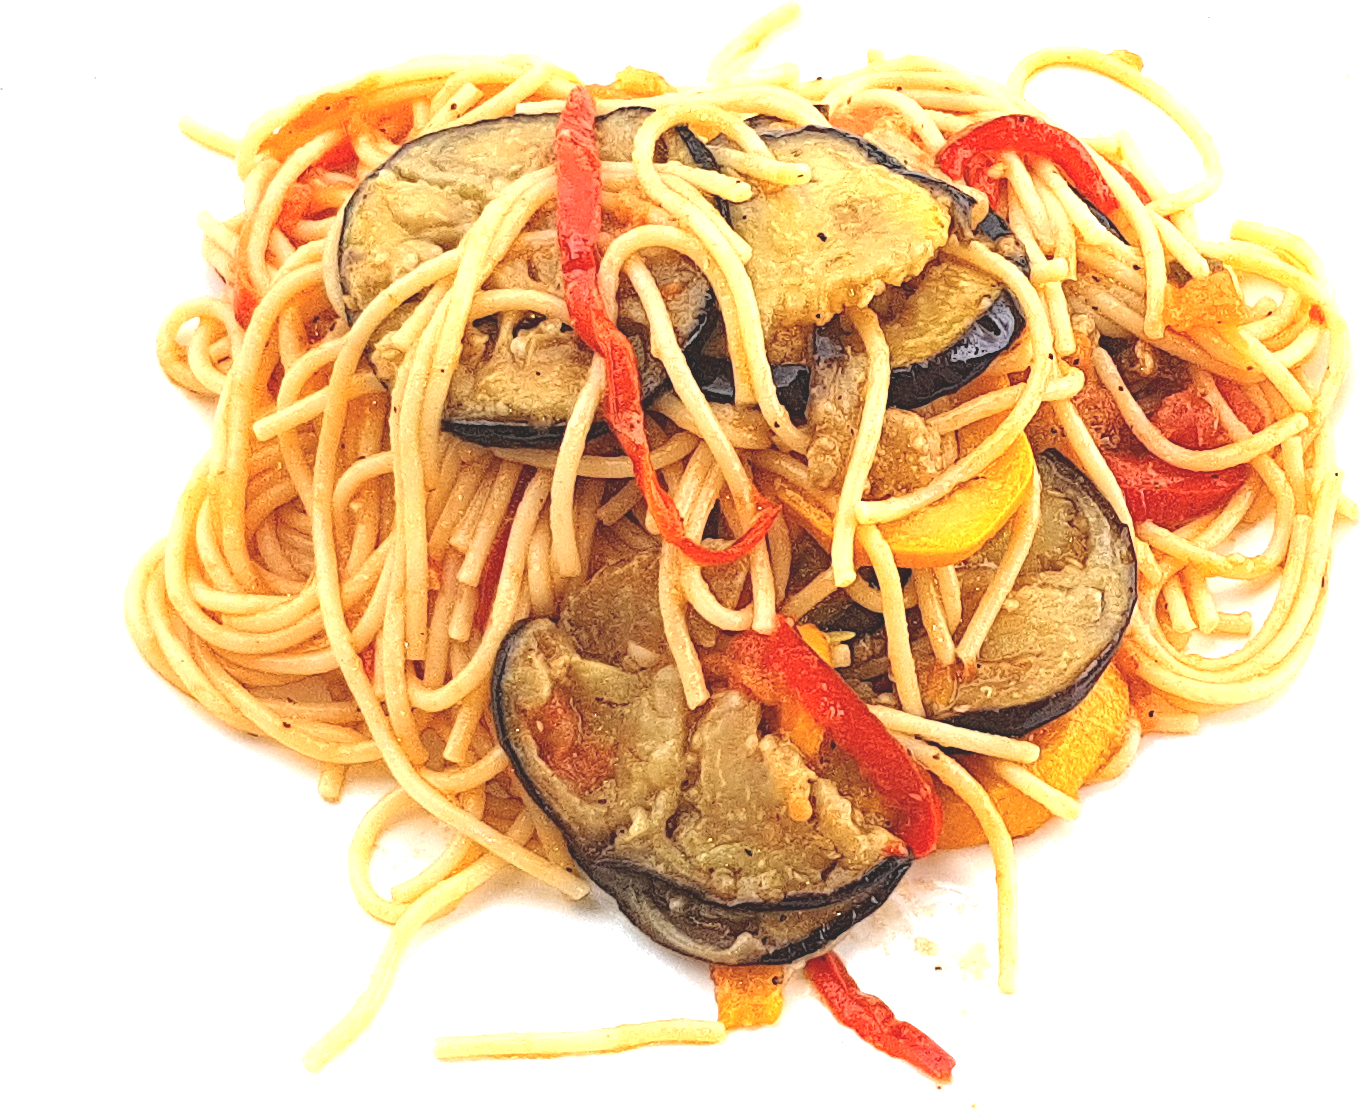
\includegraphics[width=0.8\textwidth]{fotos/spaguetti_veduras.png}
\end{center}
